\documentclass{beamer}
\title{Linear skalalering av instrumentsignaler}
\author{Fred-Olav}
\begin{document}
\maketitle

\begin{frame}
	\frametitle{Fra Temperatur til viserutslag}

	
	$$\includegraphics[width=0.8\textwidth]{current60.eps}$$

\end{frame}
\begin{frame}
	\frametitle{I reguleringssløyfe}

	
	$$\includegraphics[width=0.5\textwidth]{current02.eps}$$

\end{frame}
\begin{frame}
	\frametitle{Forholdet mellom 4-20mA og instrumentmålinger}

	
	$$\includegraphics[width=0.5\textwidth]{current42.eps}$$

\end{frame}

\begin{frame}
	\frametitle{Linear konvertering}

	
	$$\includegraphics[width=0.5\textwidth]{current43.eps}$$

	$$\dfrac{x-x_{start}}{x_{range}}=\dfrac{y-y_{start}}{y_{range}}$$\\
\end{frame}

\begin{frame}
	\frametitle{Eksempel med regulator og ventil}

	

	$$\includegraphics[height=0.3\textheight]{current44.eps}$$


\noindent
	\textit{En regulator sender en strøm på 8.55mA til en direktevirkende reguleringsventil (4mA er lukket og 20mA er åpen. Hvor åpen(0-100\%) skal reguleringsventilen være med dette strømsignalet? }

\vskip 10pt

%To solve for percentage of stem travel ($x$) at 8.55 milliamps of signal current ($y$), we may use the linear equation developed previously to predict current in milliamps ($y$) from signal value in percent ($x$):

\end{frame}

	\begin{frame}
		\frametitle{Eksempel med regulator og ventil}

		
	$$\includegraphics[width=0.8\textwidth]{current43x01.eps}$$

	\end{frame}





\vskip 10pt



\begin{frame}
	\frametitle{Utregning}

	\begin{align*}
		\dfrac{x-x_{start}}{x_{range}}&=\dfrac{y-y_{start}}{y_{range}}\\
		\dfrac{x-0}{100}&=\dfrac{8.55-4}{16}\\
		x&=\dfrac{4.55}{16}\cdot 100\\
		x&=28.4\\
	\end{align*}
	

\end{frame}



















\end{document}
